\chapter*{Ringraziamenti}
\addcontentsline{toc}{chapter}{Ringraziamenti}
%Corpo dei ringraziamenti
Questa tesi è stata resa possibile dal contributo nella mia vita di tante persone, che giorno per giorno mi hanno sempre dato il loro sostegno, a voi dedico questa mia Tesi.\\
Un ringraziamento speciale alla mia famiglia, in particolare a mia \textbf{Madre} e mio \textbf{Padre}: è grazie al vostro sostegno e incoraggiamento se oggi sono riuscito a raggiungere questo traguardo.\\
La forza di arrivare qui, oggi, però non è dovuta solo a loro, devo per forza ringraziare dell'affetto e il sostegno speciale da parte dei miei cari amici, che ogni giorno hanno condiviso con me gioie, sacrifici e successi, senza voltarmi mai le spalle, mi hanno dato la forza di arrivare a questo prezioso traguardo.
\textbf{Filippo}, \textbf{Gabriele}, \textbf{Marta}, grazie di TUTTO.\\
Un pensiero in particolare vola verso la mia dolce \textbf{\textit{Nicoleta}}, è sicuramente grazie all'affetto e le attenzioni che mi hai donato che sono riuscito a tenere dritto il timone ed arrivare qui oggi.
Per terminare voglio ringraziare tutti i professori che negli ultimi 18 anni hanno guidato il mio cammino, loro che hanno sempre creduto in me e nelle mie capacità. Un ringraziamento più speciale va però alla mia professoressa e mentore \textbf{Beniamina Rauch} che fu la prima a vedere il mio potenziale e coltivarlo.\\
Oltre a lei ringrazio il mio relatore \textbf{Daniele Carnevale} che in questi anni universitari, da quando mi ha conosciuto, ha sempre creduto in me e mi ha permesso di fare esperienze che mai avevo immaginato.\\ \\
Un sentito grazie a tutti voi.\\
%%TODO: Aggiungere firma con tavoletta frafica
%
\chapter*{Introduzione}
\addcontentsline{toc}{chapter}{Introduzione}
Il presente lavoro di tesi si colloca nel contesto delle tecniche di controllo per impianti Tokamak come
FTU (Frascati Tokamak Upgrade), attualmente in smaltimento, Proto-Sphera o ITER (International Thermonuclear Experimental Reactor).\\
La tesi è stata realizzata in collaborazione con il centro ricerche ENEA (Ente Nazionale per l’Energia e l’Ambiente) di Frascati è incentrata sullo sviluppo e creazione del prototipo di controllo delle bobine magnetiche che permettono il controllo e confinamento magnetico del plasma all'interno dell'impianto Tokamak.

\section*{Fusione Termonucleare}
\addcontentsline{toc}{section}{Fusione Termonucleare}
In fisica nucleare la fusione è il processo mediante il quale i nuclei di due o più atomi vengono compressi tanto da far prevalere l’interazione forte sulla repulsione coulombiana, unendosi tra loro e andando così a formare un nucleo di massa minore della massa dei reagenti con la conseguente liberazione di un’elevata quantità di energia che conferisce al processo caratteristiche fortemente esotermiche.\\
La massa mancante viene trasformata in energia in accordo con l’equazione di Einstein:
\begin{center}
	$E = (m_r - m)c^2$
\end{center}
Dove $ m_r $ è la massa dei reagenti e $ m $ è la massa risultante.\\
Il processo di Fusione Nucleare avviene naturalmente all'interno delle stelle, e trasforma l'idrogeno di cui sono composte in elio.\\
L'energia nucleare di questo prodotta da questa reazione è elevatissima e di forte interesse, anche ambientale. Tra i maggiori vantaggi troviamo:
\begin{enumerate}
	\item Il combustibile (idrogeno e deuterio) è praticamente inesauribile ed è a disposizione di tutte le nazioni che abbiano uno sbocco sul mare. Il deuterio può essere estratto dall'acqua, anche se con costi energetici non indifferenti; per fare un esempio, un ditale pieno di deuterio equivale a 20 tonnellate di carbone in termini di energia. Un lago di medie dimensioni contiene deuterio sufficiente a rifornire una nazione di energia per secoli utilizzando la fusione nucleare (ovviamente supponendo di sfruttarlo tutto).
	\item Nessuna possibilità di incidenti come quelli di Černobyl' o di Three Mile Island in quanto il reattore non contiene sostanze radioattive come l'uranio o le scorie di fissione. In oltre, possibili incidenti, come fughe di trizio o perdite di liquido refrigerante, avrebbero un impatto ambientale e radiativo molto più contenuto e temporaneo.
	\item Nessun prodotto chimico da combustione (anidride carbonica ad esempio) come residuo immesso nell'atmosfera e quasi nessun contributo al riscaldamento del pianeta.
	\item Impossibilità di utilizzo dei reattori per la produzione di materiale per scopi bellici o terroristici
	\item Basso livello di radioattività residua e produzione di sostanze con breve vita media (tempo in cui la radioattività si riduce rapidamente).
\end{enumerate}
\noindent
Tutti questi vantaggi rendono lo sviluppo di Centrali termonucleari a \textbf{Fusione Nucleare} di grande interesse e tecnologie chiave per preservare l'ambiente del nostro pianeta.\\
In questa tesi faremo riferimento a impianti sperimentali di tipo Tokamak, che però, va specificato essere solo uno dei design attualmente in sviluppo nelle ricerche sulla Fusione Nucleare controllata.
\newpage

\section*{Struttura di un Tokamak}
\addcontentsline{toc}{section}{Struttura di un Tokamak}
Un \textbf{Tokamak} (acronimo russo per "camera toroidale magnetica") è una macchina di forma toroidale (a ciambella) in cui un gas (solitamente idrogeno) viene portato nello stato di plasma e mantenuto coeso e lontano dalle pareti interne grazie ad un campo magnetico creato da elettromagneti esterni alla camera.
\begin{figure}[h]
	\centering
	\caption[\citefield{ACS770}{series} Schema di collegamento dal Datasheet]{Collegamento dal Datasheet}
	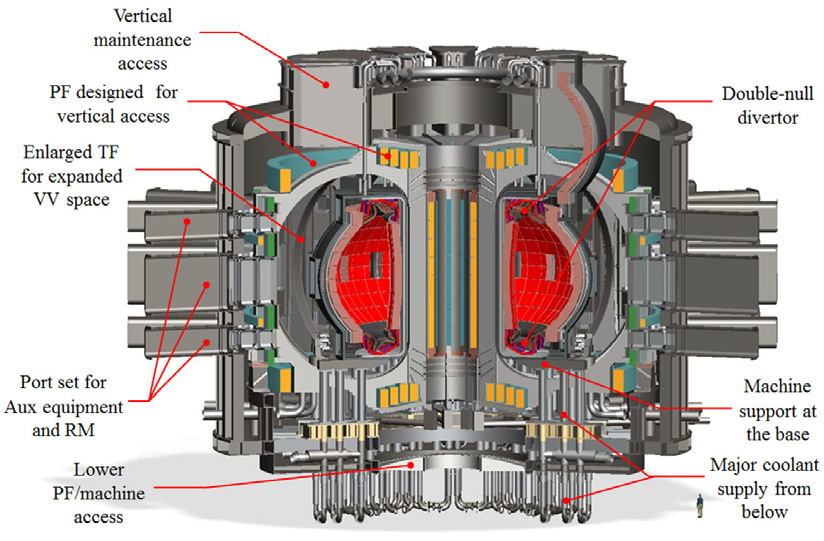
\includegraphics[width=0.65\textwidth]{Introduzione/K-DEMO_device_core_design_features.jpg}
\end{figure}

\noindent
La forma del Tokamak a toro (ciambella) è studiata per permettere alle particelle del plasma di muoversi all'interno del campo magnetico, creato all'esterno delle pareti (\textit{Esterno Vessel}) in un moto circolare.\\
Questo movimento avviene poiché le particelle del plasma sono per definizione cariche, e in quanto tali, se immerse in un campo magnetico esse tendono a muoversi seguendo una traiettoria elicoidale (detta anche moto di ciclotrone) attorno alle linee del campo magnetico, che in questo caso sono chiuse e contenute all'interno della sezione del Tokamak (\textit{Interno Vessel}).\\
L'uso di una confinazione magnetica per questo plasma è dovuta all'impossibilità, per qualunque materiale, di resistere alle enormi temperature raggiunte dal plasma durante la fusione in un contatto diretto con esse.\\
Grazie all'equazione di Larmor, che definisce il raggio di Larmor:\\
\begin{vwcol}[widths={0.3,0.7}, sep=8mm, rule=1px]
	\begin{empheq}[box=\mathCalc]{equation*} \label{eq:Larmor}
		{\displaystyle \,\rho ={\frac {mv_{\perp }}{Ze\,B}}}
	\end{empheq}
	\newpage % con wcol, le colonne sono "pagine"
	\begin{spacing}{1.25}
		{\footnotesize
			$ {\displaystyle v_{\perp }} $ è la velocità della particella perpendicolare al campo magnetico.\\
			$ {\displaystyle m} $ è la sua massa.\\
			$ {\displaystyle B} $ è l'intensità del campo magnetico.\\
			$ {\displaystyle Ze} $ è la carica del portatore.
		}
	\end{spacing}
\end{vwcol}

\noindent
Abbiamo che questo "\textbf{Tubo}" di plasma, contenuto all'interno del Vessel, non si può espandere più di $ {\displaystyle \rho } $ dalla linea di campo.\\
Ciò rende un campo magnetico il mezzo ottimo per confinare in modo efficiente un plasma, e i Tokamak sono impianti progettati per creare questo confinamento in maniera efficace e sicura, cercando al tempo stesso di compattare il plasma su se stesso (aumentando il campo magnetico $ {\displaystyle B} $), e conseguentemente avvicinando gli atomi tra loro (riduzione di $ {\displaystyle \rho } $), aumentando così la probabilità di ottenere una reazione di fusione. 

\section*{Obiettivi della Tesi}
\addcontentsline{toc}{section}{Obiettivi della Tesi}
L'obiettivo della tesi è sviluppare il prototipo della scheda di controllo delle bobine, in grado di ricevere comandi attraverso la rete di interconnessione tra i dispositivi di controllo dell'impianto Tokamak, qui pensata per Inter-operare con il Framework MARTe2, e attuare un controllo rapido sulla corrente della bobina seguendo tali riferimenti.\\